Analisis hasil pengujian berisi analisis terhadap hasil pengujian yang telah dilakukan. Analisis dilakukan dengan membandingkan hasil pengujian dengan spesifikasi kebutuhan yang telah ditetapkan sebelumnya. Apabila hasil pengujian sesuai dengan spesifikasi kebutuhan, maka sistem dapat dikatakan berhasil. Sebaliknya, apabila hasil pengujian tidak sesuai dengan spesifikasi kebutuhan, maka sistem dapat dikatakan gagal.
Dalam melakukan analisis hasil pengujian, dapat digunakan beberapa metode, yaitu:
Confusion Matrix: Implementasi confusion matrix membantu memahami sejauh mana model dapat mengidentifikasi True Positives (mesin yang diakui dengan benar), True Negatives (mesin yang ditolak dengan benar), False Positives (mesin yang salah diakui), dan False Negatives (mesin yang salah ditolak).

\begin{figure}
	\centering
	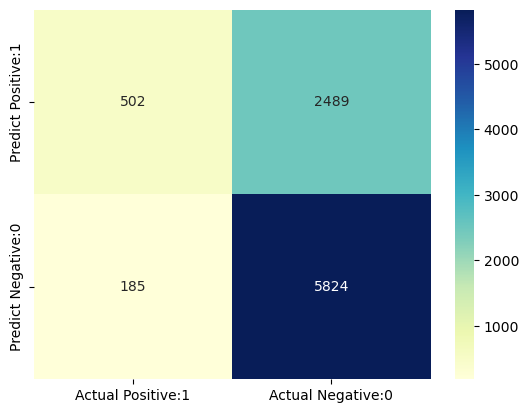
\includegraphics[width=0.5\textwidth]{BAB_TESIS/IMAGES/confusion_matrix.png}
	\caption{Confusion Matrix}
	\label{fig:confusion_matrix}
\end{figure}

\begin{table}[H]
	\caption{Confusion Matrix}
	\centering
	\begin{tabular}{|c|c|c|}
		\hline
		& \textbf{Predicted: 0} & \textbf{Predicted: 1} \\
		\hline
		\textbf{Actual: 0} & True Negative & False Positive \\
		\hline
		\textbf{Actual: 1} & False Negative & True Positive \\
		\hline
	\end{tabular}
	\label{table:1}
\end{table}

Hasil tertinggi yang diperoleh dari Tabel \ref{table:sampel_hasil_pengujian_random_forest} adalah sebagai berikut:

\begin{table}[H]
	\caption{Hasil Pengujian Random Forest}
	\centering
	\begin{tabular}{|c|c|}
		\hline
		\textbf{Parameter} & \textbf{Values} \\
		\hline
		n\_estimators & 500 \\
		\hline
		max\_depth & None \\
		\hline
		min\_samples\_split & 2 \\
		\hline
		min\_samples\_leaf & 2 \\
		\hline
	\end{tabular}
	\label{table:hasil_rf}
\end{table}

Dengan hasil sebagai akurasi 0.708, presisi 0.701, recall 0.968, dan F1 score 0.813. Dengan hasil ini diperoleh akurasi yang lebih rendah dari yang diharapkan. Hal ini disebabkan oleh dataset yang digunakan tidak seimbang. Dengan demikian, model yang dihasilkan cenderung memprediksi kelas mayoritas. Untuk membuktikan hal ini, dapat dilakukan pengecekan dengan melihat presentase target pada dataset. Berikut adalah presentase target pada dataset